\documentclass[a4paper, 12pt]{article}
\usepackage[left=2cm, right=2cm, top=2cm, bottom=2cm]{geometry}
\setlength{\parindent}{0cm}
\usepackage{graphicx}
\begin{document}
\title{ME20B088}
\author{Jay Harish Shah}
\date{\today}
\maketitle

\tableofcontents

\listoffigures

\section{Jay Harish Shah, ME20B088}
Name: Jay Harish Shah
Roll No.: ME20B088

\section{Required equations}
\begin{equation}
\omega =\int_{t_1}^{t_2}{ \alpha dt}	
\label{eqn:omega}
\end{equation}

\begin{equation}
\tau = \int_{\alpha_1}^{\alpha_2}{I d\alpha}
\label{eqn:tau}
\end{equation}

\subsection{Analysis}
\begin{figure}
	\begin{center}
		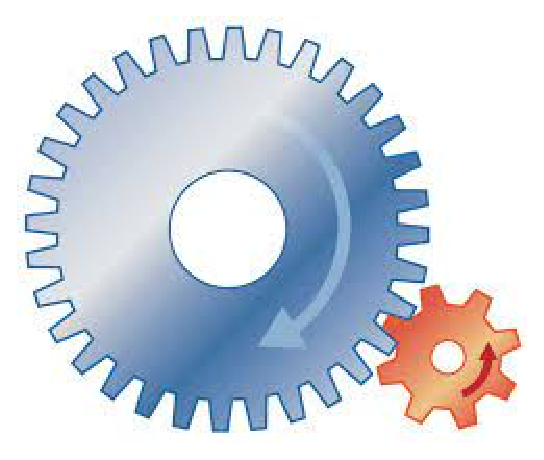
\includegraphics[scale=0.5]{me20b088.eps}
	\end{center}
	\caption{ME20B088}
	\label{fig1}
\end{figure}

In figure~\ref{fig1} we can see the mechanism of 2 gears and how each work 
by having direct dependency on the other gears dynamics.

In equation~\ref{eqn:omega} we get the relation between
angular velocity($ \omega $) and angular acceleration($ \alpha $) and time(t)
from~\cite{wu}.

In equation~\ref{eqn:tau} we get the relation between the torque($ \tau $)
and the angular acceleration($ \alpha $) 
and moment of inertia(I) from~\cite{lazarian}.
 
\bibliography{me20b088.bib}
\bibliographystyle{plain}

\end{document}
